\protect \section *{\protect \nameref  *{MechanicalOscillations}}
\begin{Solution}{8.{2}}
		\begin{enumerate*}[label=(\alph*)]
		\item $40.0$~\si{\centi\meter\per\second};
		\item $160$~\si{\centi\meter\per\square\second};
		\item $32.0$~\si{\centi\meter\per\second};
		\item $296.0$~\si{\centi\meter\per\square\second};
		\item $0.232$~s.
		\end{enumerate*}
	
\end{Solution}
\begin{Solution}{8.{4}}
		$0.628$\si{\meter\per\second}.
	
\end{Solution}
\begin{Solution}{8.{8}}
		\begin{enumerate*}[label=(\alph*)]
			\item $28.0$~mJ;
			\item $1.02$~m/s;
			\item $12.2$~mJ;
			\item $15.8$~mJ.
		\end{enumerate*}
	
\end{Solution}
\begin{Solution}{8.{9}}
		\begin{enumerate*}[label=(\alph*)]
			\item $\frac{8}{9} E$;
			\item $\frac{1}{9} E$;
			\item $x = \pm \sqrt{\frac23} A$.
		\end{enumerate*}
	
\end{Solution}
\begin{Solution}{8.{12}}
		\begin{enumerate*}[label=(\alph*)]
			\item $0.30$~m;
			\item $0.28$~s;
			\item $1.5 \cdot 10^2$~\si{\meter\per\square\second};
			\item $11$~J.
		\end{enumerate*}
	
\end{Solution}
\begin{Solution}{8.{13}}
		\begin{enumerate*}[label=(\alph*)]
			\item $1.2$~J;
			\item $50$.
		\end{enumerate*}
	
\end{Solution}
\begin{Solution}{8.{14}}
		\begin{enumerate*}[label=(\alph*)]
			\item $1.1$~m/s;
			\item $3.3$~cm.
		\end{enumerate*}
	
\end{Solution}
\begin{Solution}{8.{16}}
		$0.366$~\si{\second}.
	
\end{Solution}
\begin{Solution}{8.{17}}
		\begin{enumerate*}[label=(\alph*)]
			\item $0.53$~m;
			\item $2.1$~s.
		\end{enumerate*}
	
\end{Solution}
\begin{Solution}{8.{20}}
		$0.0653$~\si{\second}.
	
\end{Solution}
\begin{Solution}{8.{21}}
		$7\%$.
	
\end{Solution}
\begin{Solution}{8.{22}}
		\begin{enumerate*}[label=(\alph*)]
			\item $v = a_0\sqrt{\omega^2 + \beta^2}e^{-\beta t}$;
			\item $v = |v_0|  \sqrt{1 +  \left( \frac{\beta}{\omega}\right)^2}e^{-\beta t}$.
		\end{enumerate*}	
	
\end{Solution}
\begin{Solution}{8.{23}}
		\begin{enumerate*}[label=(\alph*)]
			\item $14.3$~s;
			\item $5.27$.
		\end{enumerate*}
	
\end{Solution}
\begin{Solution}{8.{24}}
		\begin{enumerate*}[label=(\alph*)]
			\item $3.16$~\si{\per\second};
			\item $6.28$~\si{\per\second};
			\item $5.09$~cm.
		\end{enumerate*}
	
\end{Solution}
\begin{Solution}{8.{26}}
		$0.641$~Hz or $1.31$~Hz.
	
\end{Solution}
\begin{Solution}{8.{28}}
		\begin{enumerate*}[label=(\alph*)]
			\item $47.9$~\si{\per\second} and $52.1$~~\si{\per\second};
			\item $1.5$~\si{\second}.
		\end{enumerate*}
	
\end{Solution}
\begin{Solution}{8.{29}}
		$y^2 = 4x^2 (1 - \frac{x^2}{a^2})$.
		
		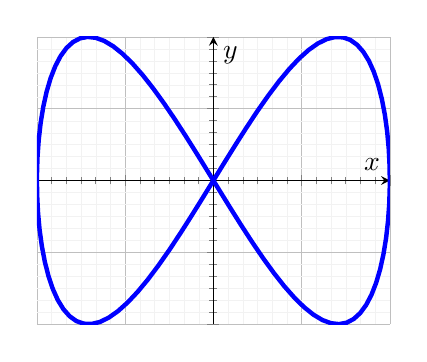
\begin{tikzpicture}
		\begin{axis}[%
		% === Налаштування сітки ===
		grid = both,
		grid style={line width=.1pt, draw=gray!10},
		major grid style={line width=.2pt,draw=gray!50},
		minor tick num = 5,
		minor grid style = {line width=.1pt,draw=gray!10},
		% === Налаштування положення координатних осей ===
		axis lines = middle,
		axis line style={-stealth},
		xticklabels = \empty,
		yticklabels = \empty,
		xlabel={$x$},
		ylabel={$y$},
		width=0.5\linewidth,
		trig format plots=rad,
		]
		\addplot [domain=0:2*pi, samples=100, blue, ultra thick] ({1*sin(x)}, {1*sin(2*x)});
		\end{axis}
		\end{tikzpicture}
	
\end{Solution}
\begin{Solution}{8.{30}}
		$y^2 = a (1 - \frac{2x^2}{a^2})$.
		
		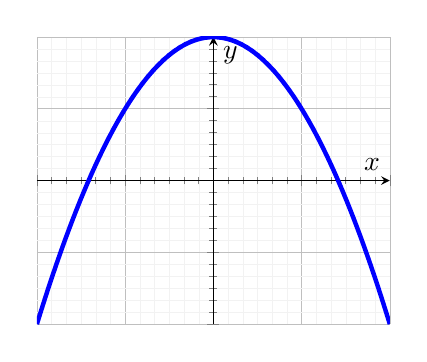
\begin{tikzpicture}
		\begin{axis}[%
		% === Налаштування сітки ===
		grid = both,
		grid style={line width=.1pt, draw=gray!10},
		major grid style={line width=.2pt,draw=gray!50},
		minor tick num = 5,
		minor grid style = {line width=.1pt,draw=gray!10},
		% === Налаштування положення координатних осей ===
		axis lines = middle,
		axis line style={-stealth},
		xticklabels = \empty,
		yticklabels = \empty,
		xlabel={$x$},
		ylabel={$y$},
		width=0.5\linewidth,
		trig format plots=rad,
		]
		\addplot [domain=0:2*pi, samples=100, blue, ultra thick] ({1*sin(x)}, {1*cos(2*x)});
		\end{axis}
		\end{tikzpicture}
	
\end{Solution}
